\lstset{
	basicstyle=\fontsize{8}{10}\linespread{0.8}\lstfont,
	language=matlab, % Или другой ваш язык -- см. документацию пакета
	commentstyle=\color{comment},
	numbers=left,
	numberstyle=\tiny,
	stepnumber=1,
	numbersep=5pt,
	xleftmargin =.19in,
	tabsize=4,
	extendedchars=\true,
	breaklines=true,
	keywordstyle=\color{blue},
	frame=single,
	stringstyle=\lstfont\color{string}\lstfont,
	showspaces=false,
	showtabs=false,
	showstringspaces=false,
	showstringspaces=false,
	inputencoding=utf8x,
	keepspaces=true,
	captionpos=t,
	breakatwhitespace=false,
}

\section{Технологическая часть}

\subsection{Выбор языка программирования и среды разработки}
Программное обеспечение разрабатывается с использованием операционной системы Ubuntu 20.04 LTS \cite{ubuntu}.

Для создания базы данных нечетких экспертных систем принято решение об использовании СУБД PostgreSQL \cite{Postgres} по следующим причинам:
\begin{itemize}
	\item максимальное соответствие стандарту SQL;
	\item открытый исходный код;
	\item поддержка БД неограниченного размера;
	\item наличие большого количества типов данных, в том числе uuid;
	\item кроссплатформенность;
	\item возможность создания пользователей на уровне БД.
\end{itemize}

Для генерации нечетких экспертных систем из исходных данных используется Matlab \cite{matlab} в связи с рядом преимуществ:
\begin{itemize}
	\item наличие пакета Fuzzy Logic Toolbox для работы с нечеткими экспертными системами типа Мамдани и Сугено:
		\begin{itemize}
			\item генерация нечетких систем на основе примеров входных и выходных данных;
			\item задание типа генерируемой экспертной системы и вида функций \\*принадлежности;
			\item изменение формы функций принадлежности; 
		\end{itemize}
	\item бесплатная лицензия для студентов;
	\item подключение к базе данных.
\end{itemize}

Приложения для работы с БД написано на языке Java \cite{Java} в соответствии с приведенными ниже соображениями:
\begin{itemize}
	\item кроссплатформенность;
	\item строгая типизация данных;
	\item автоматический сборщик мусора;
	\item компиляция в Just-in-time;
	\item большое количество расширений и библиотек.
\end{itemize}

Для создания графического интерфейса используется фреймворк JavaFX поскольку:
\begin{itemize}
	\item является кроссплатформенным;
	\item имеет утилиту Scene Builder для автоматической генерации FXML файлов разметки;
	\item поддерживает большое количество управляющих элементов.
\end{itemize}

Для редактирования кода используется среда разработки IntelliJ IDEA \cite{Idea} по нескольким причинам:
\begin{itemize}
	\item встроенная утилита Scene Builder для работы с фреймфорком JavaFX;
	\item глубокий анализ кода, поддержка автодополнений;
	\item наличие инструментов для работы с базами данных.
\end{itemize}

\subsection{Генерация экспертных систем}
Для генерации экспертных систем на основе входных данных была написана программа в среде Matlab с интерфейсом в виде командной строки. При запуске запрашиваются необходимые для генерации экспертной системы данные (количество выходных переменных, кластеров для каждой из них, тип создаваемой системы и путь к файлу с данными) а так же логин и пароль для подключения к БД. В программе происходит добавление данных в сами таблицы, что разрешено только для пользователей с ролью администратор. Таким образом гарантируется, что никто более не сможет создавать новые экспертные системы. Код реализованной программы приведен в листингах \ref{lst:script}--\ref{lst:script2}.

\begin{lstlisting}[caption = Программа для генерации экспертных систем на основе примеров входных и выходных данных (часть 1), label = {lst:script}]
function expert_sys_generation()
	n = input('Введите количество выходных переменных системы: ');
	mustBeInteger(n)
	if (n <= 0)
	fprintf("Количество входных переменных должно быть больше нуля\n");
	return
	end
	if (n <= 0)
	fprintf("Количество входных переменных должно быть больше нуля\n");
	return
	end
	clustNums = input('Введите количество кластеров для каждой переменной: ');
	mustBeInteger(clustNums)
	sType = input("Введите тип создаваемой системы (mamdani или sugeno): ", 's');
	if (~strcmp(sType, 'mamdani') && ~strcmp(sType, 'sugeno'))
	fprintf("Некорректный тип системы\n");
	return 
	end
	path = input("Введите путь к файлу с данными для генерации нечеткой экспертной системы: ", 's');
	
	login = input("Введите логин для подключения к базе данных: ", 's');
	password = input("Введите пароль для подключения к базе данных: ", 's');

	generateAndSaveFis(n, clustNums, sType, path, login, password)
end

function generateAndSaveFis(n, clustNums, sType, path, username, password)
	A = readmatrix(path);
	databasename = 'FuzzyDb';
	dbConnection = database(databasename,username,password);
	
	ops = genfisOptions('FCMClustering', 'FISType', sType);
	ops.NumClusters = clustNums;
	fis = genfis(A(:, 1:end - n), A(:, end - n + 1:end), ops);
	
	if (strcmp(sType, 'mamdani'))
		typeName = "Mamdani";
	else
		typeName = "Sugeno";
	end
\end{lstlisting}

\begin{lstlisting}[caption = Программа для генерации экспертных систем на основе примеров входных и выходных данных (часть 2)]
	sId = saveSystem(dbConnection, typeName);
	rIds = saveRules(dbConnection, fis, sId);
	vIds = saveAntecedents(dbConnection, fis, rIds, sId);
	if (strcmp(sType, 'mamdani'))
		saveConsequentsMamdani(dbConnection, fis, rIds, sId);
	else
		saveConsequentsSugeno(dbConnection, fis, rIds, vIds, sId);
	end
	close(dbConnection);
end
function sId = saveSystem(dbConnection, typeName)
	tablename = 'system';
	colnames = {'s_id' 's_name' 's_type' 'specialization'};
	sId = getUid();
	sName = strcat('System_', string(char(randi([33 126],1,15))));
	insertData = table(sId, sName, typeName, "physics", 'VariableNames', colnames);
	sqlwrite(dbConnection, tablename, insertData);
end

function saveConsequentsMamdani(dbConnection, fis, rIds, sId)
	for i = 1:length(fis.Outputs)
		var = fis.Outputs(i);
		vId = getUid();
		query = "insert into variable values" + "(" + vId + ", '" + ...
		var.Name + "', " + var.Range(1) + ", " + var.Range(2) + ...
		", null, " + sId + ");";
		execute(dbConnection, query);
		mIds = saveVariableMfs(dbConnection, var, vId);
		for j = 1:length(fis.Rules)
			ind = fis.Rules(j).Consequent(i);
			cId = getUid();
			query = "insert into consequent values" + "(" + cId + ", '" + ...
			mIds(ind) + "', " + rIds(j) + ");";
			execute(dbConnection, query);
		end
	end
end

function saveConsequentsSugeno(dbConnection, fis, rIds, vIds, sId)
	tablename = 'consequent';
	colnames = {'c_id' 'm_id' 'r_id' 'v_id'};
	for i = 1:length(fis.Outputs)
		var = fis.Outputs(i);
		vId = getUid();
		query = "insert into variable values" + "(" + vId + ", '" + ...
		var.Name + "', " + var.Range(1) + ", " + var.Range(2) + ...
		", null, " + sId + ");";
		execute(dbConnection, query);
		mIds = saveConsequentSugenoMf(dbConnection, var, vIds);
		for j = 1:length(fis.Rules)
			ind = fis.Rules(j).Consequent(i);
			for k = 1:length(var.MembershipFunctions(1).Parameters)
				cId = getUid();
				insertData = table(cId, mIds(ind, k), rIds(j), vId, ...
				'VariableNames', colnames);
				sqlwrite(dbConnection, tablename, insertData);
			end
		end
	end
end

function mIds = saveConsequentSugenoMf(dbConnection, var, vIds)
	mIds = zeros(length(var.MembershipFunctions), ...
	length(var.MembershipFunctions(1).Parameters) + 1, 'int32');
	for j = 1:length(var.MembershipFunctions)
		mf = var.MembershipFunctions(j);
		for k = 1:length(mf.Parameters)
			mIds(j, k) = getUid();
			if (k < length(mf.Parameters))
				query = "insert into membership_function values" + ...
				"(" + mIds(j, k) + ", '" + mf.Name + ...
				"', 'linear', " + vIds(k) + ", " + ...
				mf.Parameters(k) + ");";
			else
				query = "insert into membership_function values" + ...
				"(" + mIds(j, k) + ", '" + mf.Name + ...
				"', 'crisp', null, " + mf.Parameters(k) + ");";
				end
			execute(dbConnection, query);
		end
	end
end

\end{lstlisting}

\begin{lstlisting}[caption = Программа для генерации экспертных систем на основе примеров входных и выходных данных (часть 3), label = {lst:script2}]
function mIds = saveVariableMfs(dbConnection, var, vId)
	mIds = zeros(length(var.MembershipFunctions), 'int32');
	for j = 1:length(var.MembershipFunctions)
		mIds(j) = getUid();
		mf = var.MembershipFunctions(j);
		m = mf.Parameters(2);
		s = mf.Parameters(1) * 3;
		query = "insert into membership_function values" + ...
		"(" + mIds(j) + ", '" + mf.Name + "', 'gauss', " +  ...
		vId + ", " + m + ", " + ...
		s + ");";
		execute(dbConnection, query);
	end
end

function vIds = saveAntecedents(dbConnection, fis, rIds, sId)
	anttablename = 'antecedent';
	antcolnames = {'a_id' 'm_id'};
	ratablename = 'rule_antecedents';
	racolnames = {'r_id' 'a_id'};
	vIds = zeros(length(fis.Inputs), 'int32');
	for i = 1:length(fis.Inputs)
		var = fis.Inputs(i);
		vIds(i) = getUid();
		query = "insert into variable values" + "(" + vIds(i) + ", '" + ...
		var.Name + "', " + var.Range(1) + ", " + var.Range(2) + ...
		", null, " + sId + ");";
		execute(dbConnection, query);
		mIds = saveVariableMfs(dbConnection, var, vIds(i));
		for j = 1:length(fis.Rules)
			ind = fis.Rules(j).Antecedent(i);
			if (~antecedentExists(dbConnection, mIds(ind)))
				aId = getUid();
				insertData = table(aId, mIds(ind), 'VariableNames', ...
				antcolnames);
				sqlwrite(dbConnection, anttablename, insertData);
			else
				aId = getaId(dbConnection, mIds(ind));
			end
		insertData = table(rIds(j), aId, 'VariableNames', racolnames);
		sqlwrite(dbConnection, ratablename, insertData);
		end
	end
end

function id = getUid()
	uid = javaMethod('toString', java.util.UUID.randomUUID);
	id = javaMethod('hashCode', uid);
	if (id < 0)
		id = id * -1;
	end
end

function aId = getaId(dbConnection, m_id)
	query = "SELECT a_id " + ...
	"FROM postgres.public.antecedent " + ...
	"WHERE m_id = " + m_id;

	data = fetch(dbConnection,query);
	aId = data(1, 1).a_id;
end

function exists = antecedentExists(dbConnection, m_id)
	query = "SELECT * " + ...
	"FROM postgres.public.antecedent " + ...
	"WHERE m_id = " + m_id;
	data = fetch(dbConnection,query);
	exists = height(data) ~= 0;
end

function rIds = saveRules(dbConnection, fis, sId)
	rIds = zeros(length(fis.Rules), 'int32');
	tablename = 'rule';
	colnames = {'r_id' 's_id' 'antecedent_connection' 'weight'};
	for i = 1:length(fis.Rules)
		rIds(i) = getUid();
		if (fis.Rules(i).Connection == 1)
			conn = "and";
		else
			conn = "or";
		end
		insertData = table(rIds(i), sId, conn, fis.Rules(i).Weight, 'VariableNames', colnames);
		sqlwrite(dbConnection, tablename, insertData);
	end
end
\end{lstlisting}

\subsection{Описание интерфейса}
Интерфейс программного обеспечения для работы с базой данных  экспертных систем разделен на 3 области: слева находится список нечетких систем, в центре располагается информация о правилах логического вывода или нечетких переменных выбранной системы в зависимости от текущей вкладки, справа отображается информация о правиле вывода или переменной.

Внешний вид интерфейса при запуске приложения представлен на рисунке \ref{fig:mainmenu}. 
\begin{figure}[H]
	\centering
	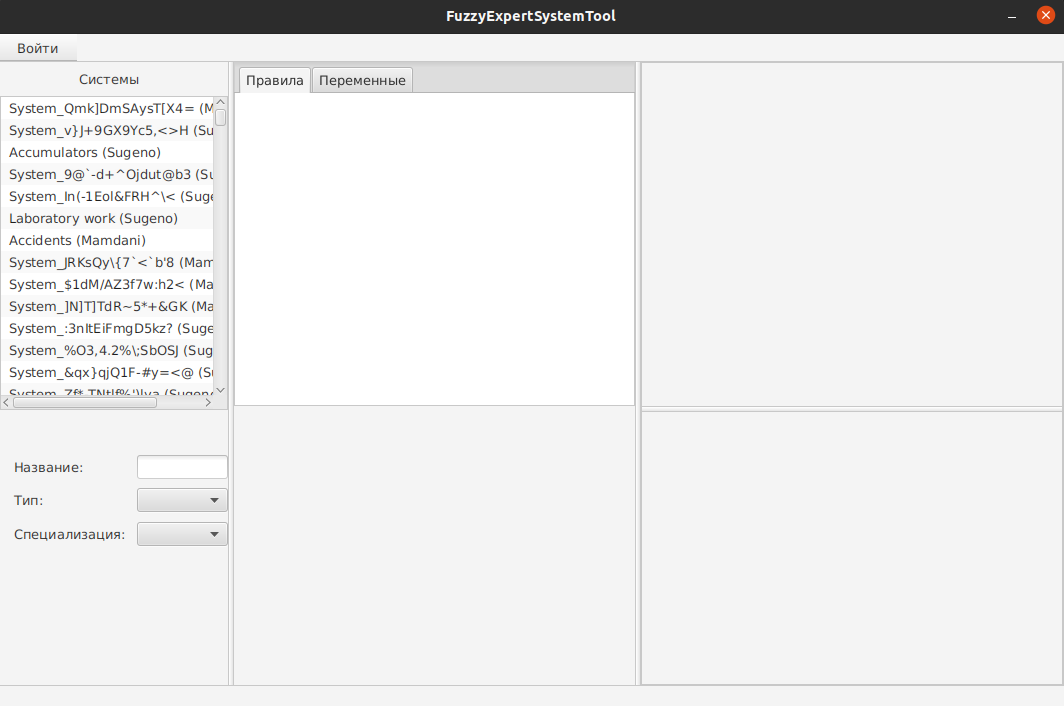
\includegraphics[width=0.7\linewidth]{img/main_menu}
	\caption{Начальное состояние приложения}
	\label{fig:mainmenu}
\end{figure}

При нажатии на имя экспертной системы снизу отображается информация о ней (имя, тип, специализация), в центре -- список определенных в ней правил логического вывода. Под списком правил находится таблица для получения результата нечеткого логического вывода текущей экспертной системы при хранящихся в базе значениях переменных. При выборе правила посредством нажатия левой кнопки мыши по соответствующей строке списка в правом верхнем углу отображается информация об антецедентах, в правом нижнем углу -- о консеквентах соответствующего правила вывода. Для отображения информации об антецеденте или консеквенте также требуется нажать на соответствующую строку левой кнопкой мыши. Пример интерфейса, отображающего информацию об антецеденте и консеквенте правила нечеткой экспертной системы представлен на \ref{fig:ruleinfo}.

\begin{figure}[H]
	\centering
	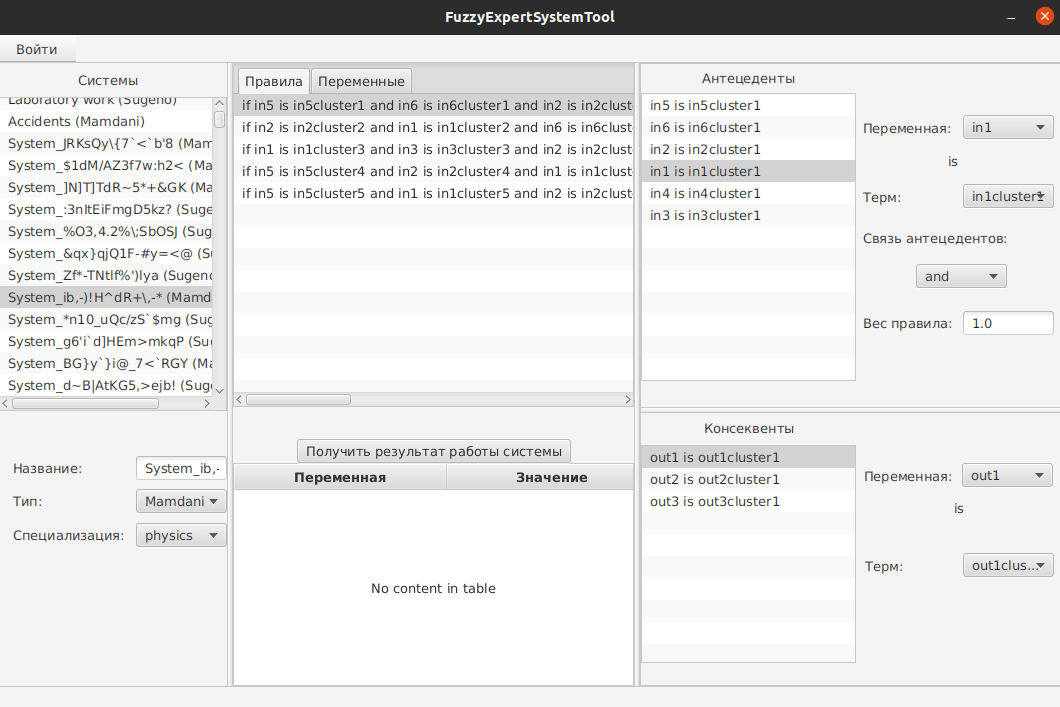
\includegraphics[width=0.7\linewidth]{img/ruleInfo}
	\caption{Информация об антецедентах и консеквентах правила нечеткого логического вывода}
	\label{fig:ruleinfo}
\end{figure}

Для получения информации о нечетких переменных необходимо нажать на соответствующую вкладку в центральной части интерфейса. При выборе нечеткой переменной снизу отображается информация о ней (название, текущее, минимальное и максимальное значения), справа появляется список функций принадлежности. При выборе функции предоставляется информация о ней и строится ее график в нижнем правом углу. Обычный пользователь может изменять текущее значение переменной для получения результата работы нечеткой экспертной системы. Пример изображения информации о переменной и ее функции принадлежности представлен на рисунке \ref{fig:varinfo}.

Для получения результата логического вывода системы необходимо изменить значения переменных на соответствующей вкладке при необходимости и нажать кнопку <<получить результат работы системы>> на вкладке правил. Пример получения результата логического вывода представлен на рисунке \ref{fig:output}.

Для подключения к базе данных с существующими учетными данными используется кнопка <<Войти>> в левом верхнем углу. При нажатии появляется всплывающее окно для ввода логина и пароля. В случае успешной аутентификации и авторизации пользователь получает сообщение об успехе, в противном случае происходит сброс текущей учетной записи до записи по умолчанию (обычного пользователя). Пример окна для ввода логина и пароля представлен на рисунке \ref{fig:authorize}.

\begin{figure}[H]
	\centering
	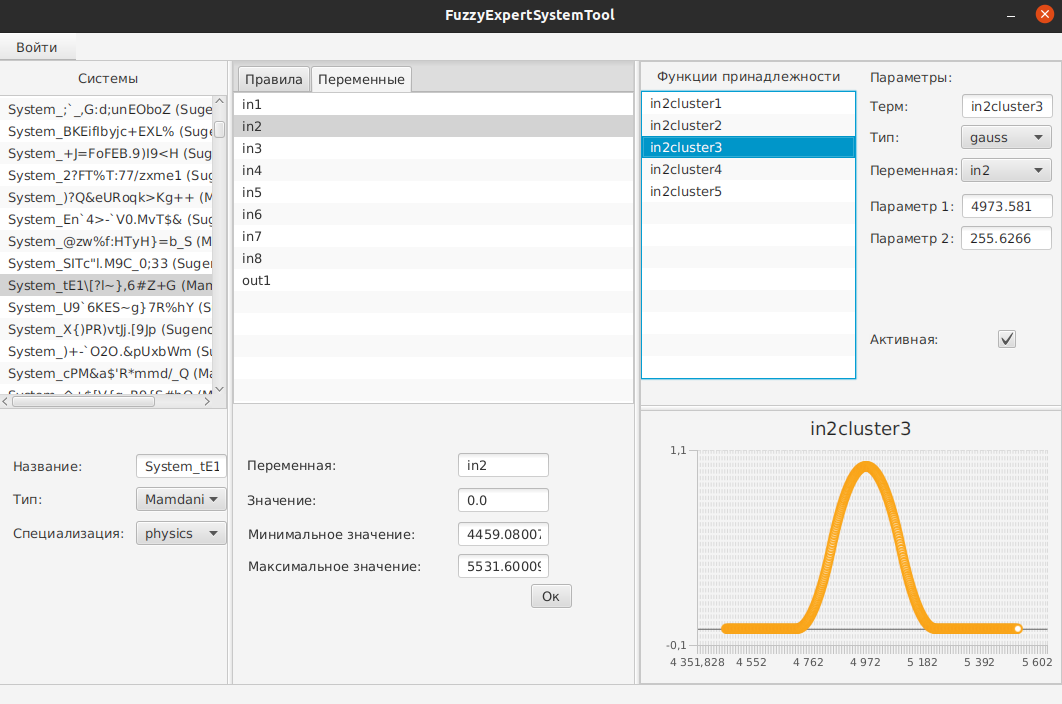
\includegraphics[width=0.7\linewidth]{img/varInfo}
	\caption{Информация о переменной системы и ее функции принадлежности}
	\label{fig:varinfo}
\end{figure}
\begin{figure}[H]
	\centering
	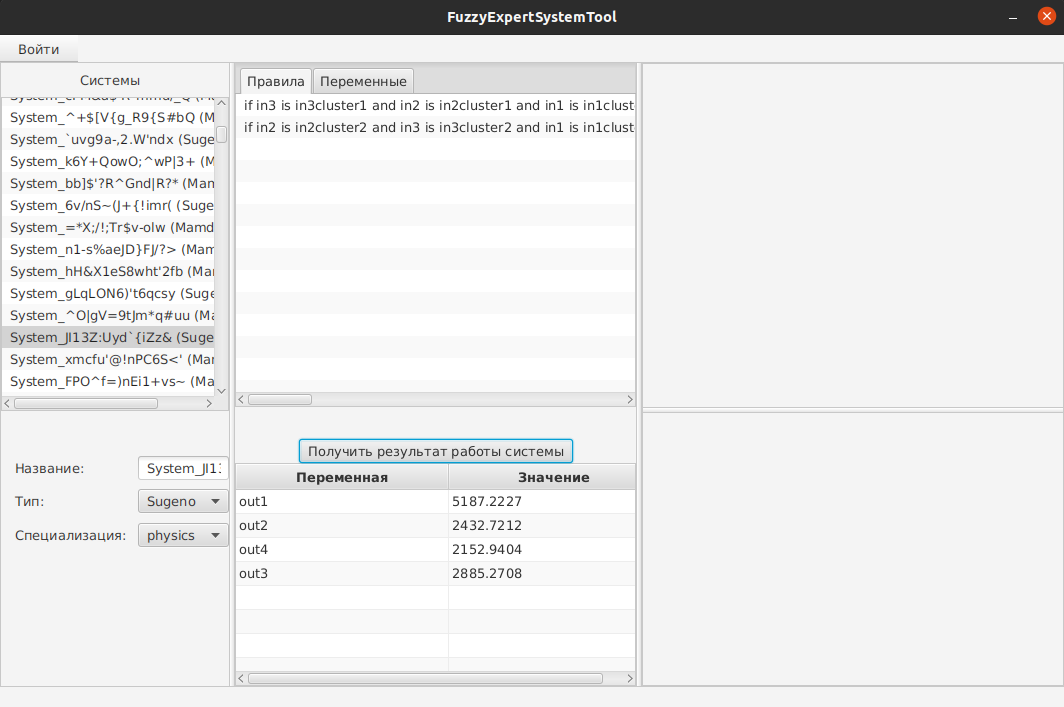
\includegraphics[width=0.7\linewidth]{img/output}
	\caption{Получение результата работы системы}
	\label{fig:output}
\end{figure}

\begin{figure}[H]
	\centering
	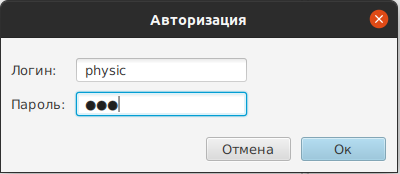
\includegraphics[width=0.4\linewidth]{img/authorize}
	\caption{Окно ввода данных для аутентификации и авторизации}
	\label{fig:authorize}
\end{figure}

При успешной авторизации пользователя с ролью администратора появляются кнопки добавления, изменения и удаления систем, правил, антецедентов, консеквентов, нечетких переменных и их функций принадлежности. При авторизации пользователя с ролью эксперта появляются кнопки добавления, изменения и удаления всех компонентов нечетких экспертных систем, специализация которых совпадает со специализацией эксперта. Эксперт не может создавать или изменять экспертные системы. Примеры интерфейсов для администратора и эксперта представлены на рисунках \ref{fig:admin}--\ref{fig:physic} соответственно. 

\begin{figure}[H]
	\centering
	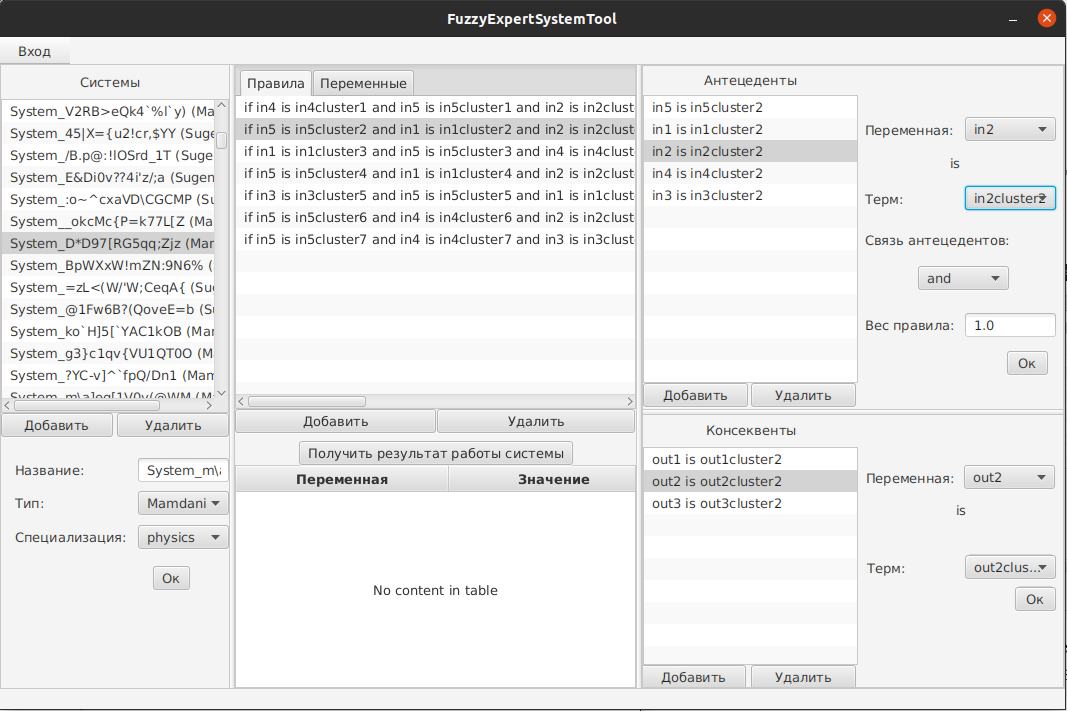
\includegraphics[width=0.7\linewidth]{img/admin}
	\caption{Пример интерфейса для пользователя с ролью администратора}
	\label{fig:admin}
\end{figure}

\begin{figure}[H]
	\centering
	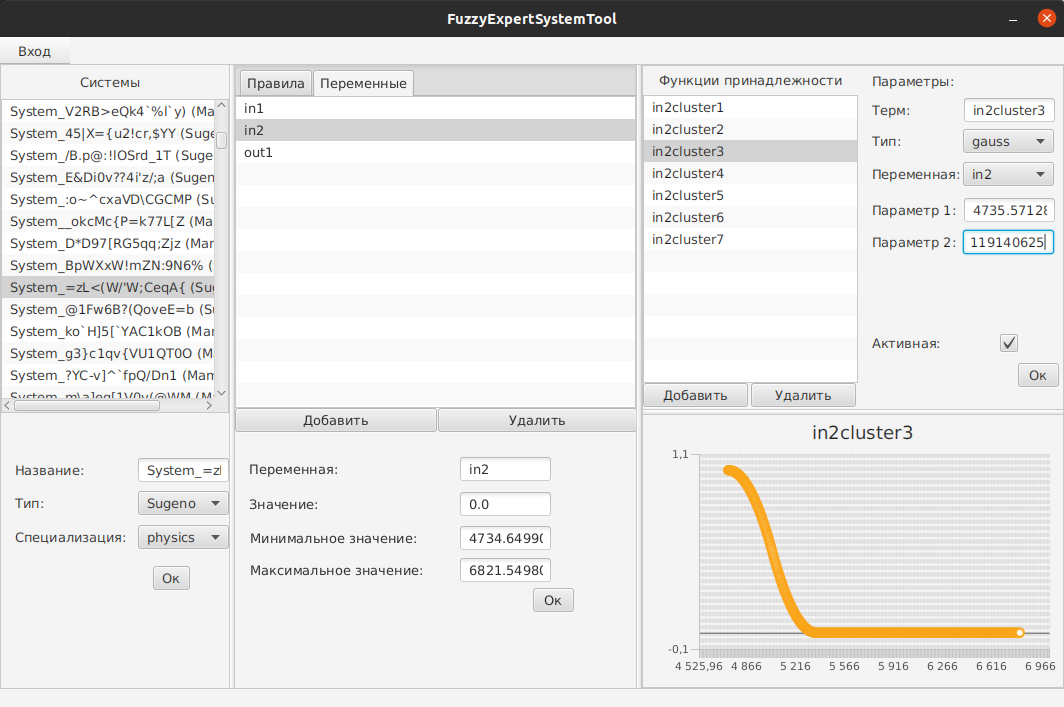
\includegraphics[width=0.7\linewidth]{img/physic}
	\caption{Пример интерфейса для пользователя с ролью эксперта в области физики}
	\label{fig:physic}
\end{figure}

\subsection{Выводы}
В данном разделе обоснован выбор средств разработки приложения, приведена программа для генерации нечетких экспертных систем, описан интерфейс приложения для работы с БД.

\pagebreak